\section{Udviklingsværktøjer}
\subsection{MATLAB}
Selve softwaren til systemet udvikles i MATLAB. Versionen der er anvendt er R2015b. Af tilføjelsespakker bruges følgenede:
\begin{itemize}
\item Arduino Support Package (14.2.2)
\item Webcam Support Package (15.2)
\end{itemize}
Disse pakker anvendes til, at interagere med Arduinoen og USB mikroskopet.

\textbf{Fritzing:} \textit{Fritzing} er brugt til at illustrere kredsløbsdiagrammer(schematics), samt enhedstest af hardwaren ved illustrationer af \textit{fumlebræt}. Dette har bidraget til dokumentationen af  enhedstestene. Derudover har det givet mulighed for at opstillingerne brugt på \textit{fumlebræt}, let kunne genskabes.

\textbf{Eagle:} \textit{Eagle} er et program til udarbejdelse af print layouts. \textit{Eagle} er brugt til at lave et samlet PCB layout for hardwareelementerne. I \textit{Eagle} er der generet Gerber-filer, som er sendt til PCB fabrikanten.

\textbf{SolidWorks:} \textit{SolidWorks} er et program til at illustrere mekaniske 3D modeller med.  \textit{SolidWorks} er brugt til at lave kamerahuset med for senere at få det 3D printet.

\textbf{Arduino IDE:} Programmet som er udbudt af \textit{Arduino} bruges til at programmere \textit{Arduino} udviklingskortet. \textit{Arduino IDE} er i projektet brugt til enhedstest for at teste hardware opstillingerne. 

\textbf{Microsoft Visio:} \textit{Microsoft Visio} er et tegne program, som bruges til at illustrere forskellige modeller. Programmet er valgt til at lave udviklingsdiagrammer, samt illustrationer med. 

\textbf{Texmaker:} Dette program er brugt til at skrive alt dokumentationen i projektet. \textit{Texmaker} gør det muligt at arbejde på samme dokument samtidigt, hvilket har været en stor hjælp.

\textbf{PivotalTracker:} \textit{PivotalTracker} er et scrumbaseret projektstyringsværktøj, der hjælper med at styre arbejdsressourcerne i projektet. Der er i afsnittet \ref{subsec:pivotalT} uddybet hvordan \textit{PivotalTracker} er brugt i projektet.

\textbf{GitHub:} Er et versionsstyringsprogram, som i projektet er brugt til versionsstyring af dokumenter og \textit{Matlab} koden til projektet. Se afsnit \ref{subsec:GitHub1} for uddybende dokumentation omkring hvordan \textit{Github} er brugt.

\textbf{Dropbox:} Det cloudbaserede delingsværktøj \textit{Dropbox} er i projektet brugt til at gemme og dele artikler, diagrammer, billeder og generelle noter.

\textbf{Microsoft Onenote:} \textit{Onenote} er et program til at lave noter i. I projektet er programmet brugt til at have fælles noter og huskelister.

\subsection{GitHub}
\label{subsec:GitHub1}
Til versionsstyring af projektdokumentationen og source kode anvendes GitHub, som bygger på open source versions styrings systemet Git. Her opdateres der løbende ændringer, så det nyeste dokumentation og source kode altid er tilgængeligt. 
Som user interface til GitHub anvendes GitHub Desktop (figur: \ref{fig:git}). I GitHub Desktop vises en tidslinje, for hvornår der er lavet ændringer. Under de enkelte filer kan man se hvad der er ændret i for den gældende version. Programmet giver yderligere indblik i hvilke filer der lokalt er lavet ændringer i, som ikke er tilføjet repositoriet endnu.
\begin{figure}[H]
	\centering
	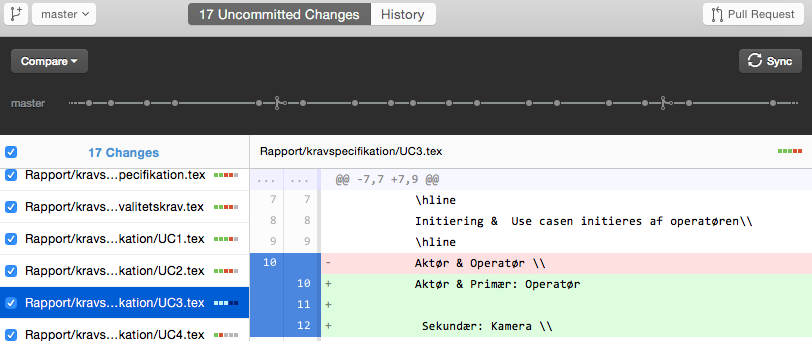
\includegraphics[width=1\textwidth]{billeder/github.png}
	\caption{GitHub Desktop}
	\label{fig:git}
\end{figure}

\newpage

\subsection{Pivotal Tracker}
\label{subsec:pivotalT}
Til projektstyring anvendes Pivotaltracker, som er et online værktøj baseret på SCRUM. I Pivotaltracker defineres projektets arbejdsopgaver, hvorefter de tildeles point alt efter hvor stor arbejdsbyrden er. De enkelte opgaver prioriteres herefter i projektets backlog, hvor Pivotaltracker automatisk tilføjer opgaver til den igangværende sprint udfra den nuværende “velocity”. En ny sprint påbegyndes automatisk når en ny uge starter.

Det betyder, at der er fuldstændig styr på om projektet går for langsomt, eller om udviklingen af projektet er godt med. Dette kan sammenlignes med gatestate arbejdsmetoden, hvor der er flere deadlines end der vil være i for eksempel vandfaldsmetoden.

Herudover giver Pivotaltracker mulighed for en komplet log over projektets udførte opgaver og afsluttede sprints. Her kan man se hvilke opgaver der er udført i hvilken uge. I projektet anvendes dette som logbog over udførte arbejdsopgaver.

En opgave kan have forskellige states, som definerer dens status. Når en opgave er afsluttet kan den afleveres til review, hvor den herefter enten kan godkendes eller afvises. Dette er særligt anvendeligt i projektets udviklingsfase, hvor en feature kan testes og godkendes af et andet projektmedlem. Figur \ref{fig:pt_sprints}  viser et overblik over tidligere sprints, hvor figur \ref{fig:pt_currentsprint} viser en igangværende sprint med opgaver der er godkendte, afsluttet og ikke færdiggjorte endnu.

\begin{figure}[htbp] \centering
\begin{minipage}[b]{0.48\textwidth} \centering
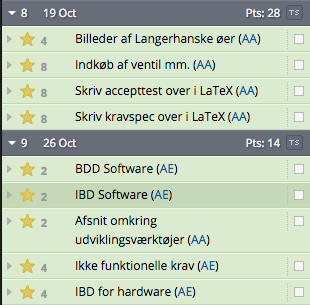
\includegraphics[width=1.00\textwidth]{billeder/pt_previous_sprints} % Left picture
\end{minipage} \hfill
\begin{minipage}[b]{0.48\textwidth} \centering
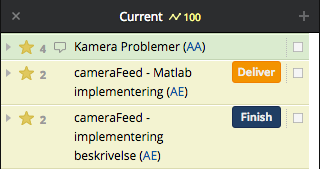
\includegraphics[width=1.00\textwidth]{billeder/pt_current_sprint} % Right picture
\end{minipage} \\ % Captions og labels
\begin{minipage}[t]{0.48\textwidth}
\caption{Færdiggjorte sprints} % Left caption and label
\label{fig:pt_sprints}
\end{minipage} \hfill
\begin{minipage}[t]{0.48\textwidth}
\caption{Igangværende sprint} % Right caption and label
\label{fig:pt_currentsprint}
\end{minipage}
\end{figure}

